\section{nyt afsnit om overbelægning - udkast}

Noget indledende tekst. 

\begin{figure}[H]
	\flushleft 
	\caption{Belægningsgrad i procent på ortopædkirugisk afdeling}
	\centering
	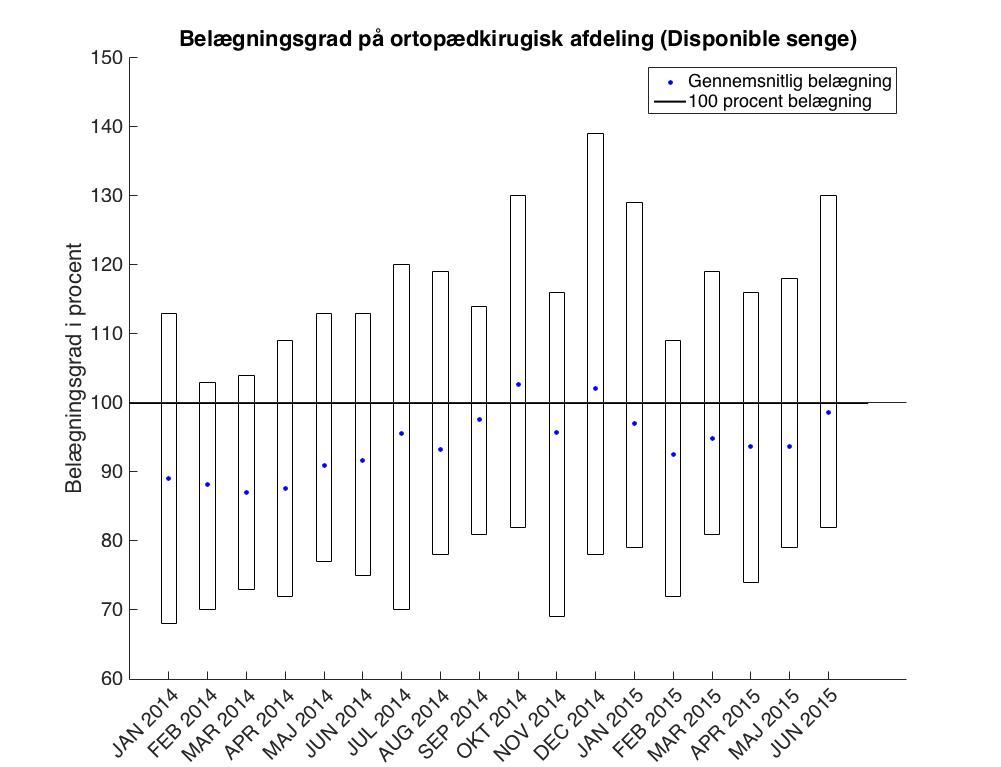
\includegraphics[scale=.5]{figures/maxminoverbelaeg.png}
	\label{maxminbelaeg}
	\flushleft
	\textit{Figuren viser minimums- og maksimumsbelægning på ortopædkirugisk, samt den gennemsnitlige belægning, fra januar 2014 til juni 2015 på ortopædkirugisk afdeling på Aalborg Universitetshospital.}
\end{figure}

Som det ses på \figref{maxminbelaeg} er den gennemsnitlige belægning på ortopædkirugisk afdeling typisk under $100$\%. Kun $2$ ud af $18$ måneder har en gennemsnitlig belægning over $100$\%. Det ses ligeledes at den maksimale belægning er over $100$\% i alle $18$ måneder. Dette tyder på at overbelægningen sker som spidsbelastninger.\fxnote{noget om spidsbelastninger}.

Foruden belægningsgraden er det interessant at undersøge hyppigheden. \Figref{antaldage} viser antallet af dage, hvor ortopædkirugisk afdeling på Aalborg Universitetshospital har haft en belægningsgrad over $100$\%\fxnote{alle data er fra sundhedsdatastyrelsen}

\begin{figure}[H]
	\flushleft 
	\caption{Antal dage med belægningsgrad over $100$\% på ortopædkirugisk afdeling}
	\centering
	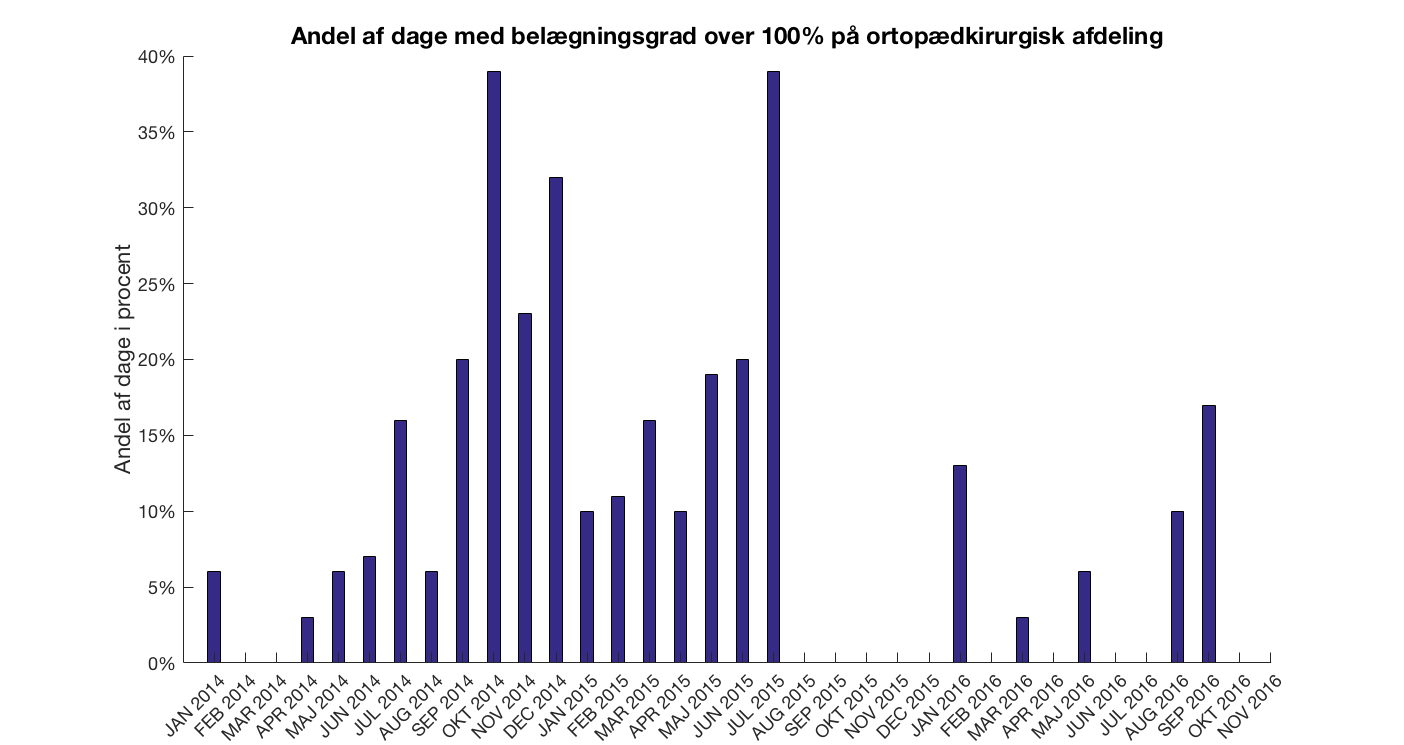
\includegraphics[scale=.5]{figures/antaldage.png}
	\label{antaldage}
	\flushleft
	\textit{Figuren antal dage med belægningsgrad over $100$\%, fra januar 2014 til juni 2015 på ortopædkirugisk afdeling på Aalborg Universitetshospital.}
\end{figure}